\documentclass{beamer}
\usepackage[utf8]{inputenc}
\usepackage[T1]{fontenc}
\usepackage{graphicx}
\usepackage{booktabs}
\usepackage[italian]{babel}
\usepackage{caption}
\usepackage{subcaption}
\usepackage{wrapfig}
\usepackage{array}
\usepackage{mathtools}

\usefonttheme{professionalfonts}
\setbeamertemplate{navigation symbols}{}
\setbeamertemplate{footline}[frame number]
\captionsetup[figure]{labelformat=empty}
\captionsetup[table]{labelformat=empty}
\captionsetup[subtable]{labelformat=empty}

\title[Misure in sistemi di sorveglianza]{Misura di posizione e velocità in sistemi di sorveglianza stradale}
\author{Nicola Sansoni}
\date[A.Y. 2020/2021]{ACADEMIC YEAR 2020/2021}
\institute[UniCa]{
    Università degli Studi di Cagliari \\
    Facoltà di Scienze \\
    Corso di Laurea Triennale in Informatica
}
\logo{
    
\includegraphics[height=1cm] {
        % images/simbolo_unica.jpg
        images/logo.png
    }
}

\begin{document}
    \frame{\setlength{\parskip}{0pt}
\vspace{2.4em}
\begin{center}
    \usebeamercolor[fg]{title}
    \usebeamerfont{title}
    % \bfseries
    \inserttitle
\end{center}

\vspace{.3em}

\begin{center}
    \usebeamerfont{author}
    {
    \small
    \usebeamercolor[fg]{title} 
    % \bfseries
    Candidato:

    }
    {
    \usebeamercolor[fg]{author}
    \insertauthor
    }
\end{center}

\begin{center}
    \usebeamercolor[fg]{institute}
    \usebeamerfont{institute}
    \insertinstitute
\end{center}

\vspace{1.2em}

\begin{columns}
    \small
    \begin{column}{.5\textwidth}
        \centering
        {
            \usebeamercolor[fg]{title} 
            % \bfseries
            Relatore:
        }

        Dott. Alessandro Sebastian Podda

    \end{column}
    \begin{column}{.5\textwidth}
        \centering
        {
            \usebeamercolor[fg]{title}
            % \bfseries
            Co-Relatore:
        }

        Prof. Salvatore M. Carta
    \end{column}
\end{columns}

\vspace{2.4em}

\begin{center}
    \usebeamercolor[fg]{date}
    \usebeamerfont{date}
    \insertdate
\end{center}
}

    \setcounter{part}{-1}
    \part{Introduzione}
    \section{Contesto}
    \frame{
        \frametitle{\insertsection}
        Vista l'alta diffusione di telecamere di sorveglianza nelle città, è d'interesse lo sviluppo di un sistema di sorveglianza intelligente che sia in grado di rilevare situazioni di rischio.
        \vfill
        Per valutare il rischio è utile conoscere posizione e velocità delle entità inquadrate dalle telecamere, così da poter comprenderne il comportamento.
        \vfill
        Misurare queste grandezze direttamente sull'immagine porta a risultati poco utili, in quanto queste misure soffrono di distorsione prospettica e rumore.
        Vogliamo presentare delle tecniche per la correzione di queste problematiche.
    }

    \section{Obiettivi della tesi}
    \frame{
        \frametitle{\insertsection}
        Vogliamo individuare delle metodologie efficaci per correggere la distorsione prospettica e il rumore, così da poter misurare la posizione e la velocità delle entità inquadrate.
    }

    \section{Attività svolte}
    \frame{
        \frametitle{\insertsection}
        \begin{itemize}
            \item Studio delle trasformazioni di proiezione
            \item Sviluppo di un algoritmo di correzione del rumore
            \item Implementazione delle tecniche scelte in un sistema di sorveglianza stradale
        \end{itemize}
    }

    \part{Posizione}
    \frame{\partpage}
    \section{Geometria della scena}
    \frame{
        \frametitle{\insertsection}

        \begin{columns}
            \begin{column}[]{.66\textwidth}

                Per comprendere la posizione delle entità è necessario conoscere lo spazio in cui queste si muovono.
                \vspace{1.2em}

                A noi interessano entità che si muovono su strade e marciapiedi.
                Possiamo approssimare questo spazio con un piano.
                \vspace{1.2em}

                Dobbiamo quindi trovare una trasformazione che corregga la nostra inquadratura, permettendoci di ottenere la posizione delle entità sul piano stradale dalla loro posizione nell'immagine.

            \end{column}
            \begin{column}[c]{.33\textwidth}
                \centering
                \footnotesize
                \itshape
                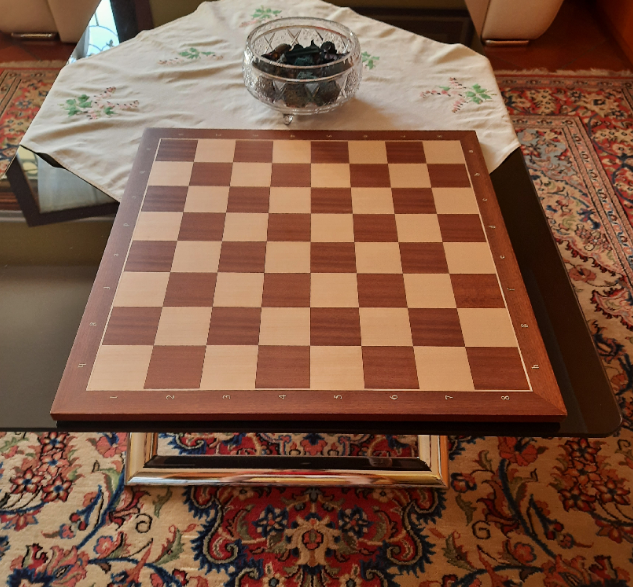
\includegraphics[height=\textheight, width=\textwidth, keepaspectratio]
                { images/persp1.png } \\
                Inquadratura originale \\
                \vspace{1.2em}
                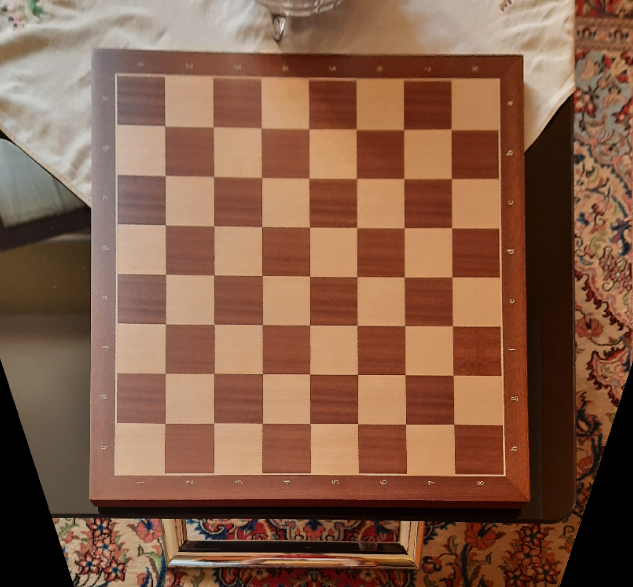
\includegraphics[height=\textheight, width=\textwidth, keepaspectratio]
                { images/persp2.png } \\
                Inquadratura corretta \\
            \end{column}
        \end{columns}
    }

    \section{Proiezione sul piano}
    \frame{
        \frametitle{\insertsection}

        \centering
        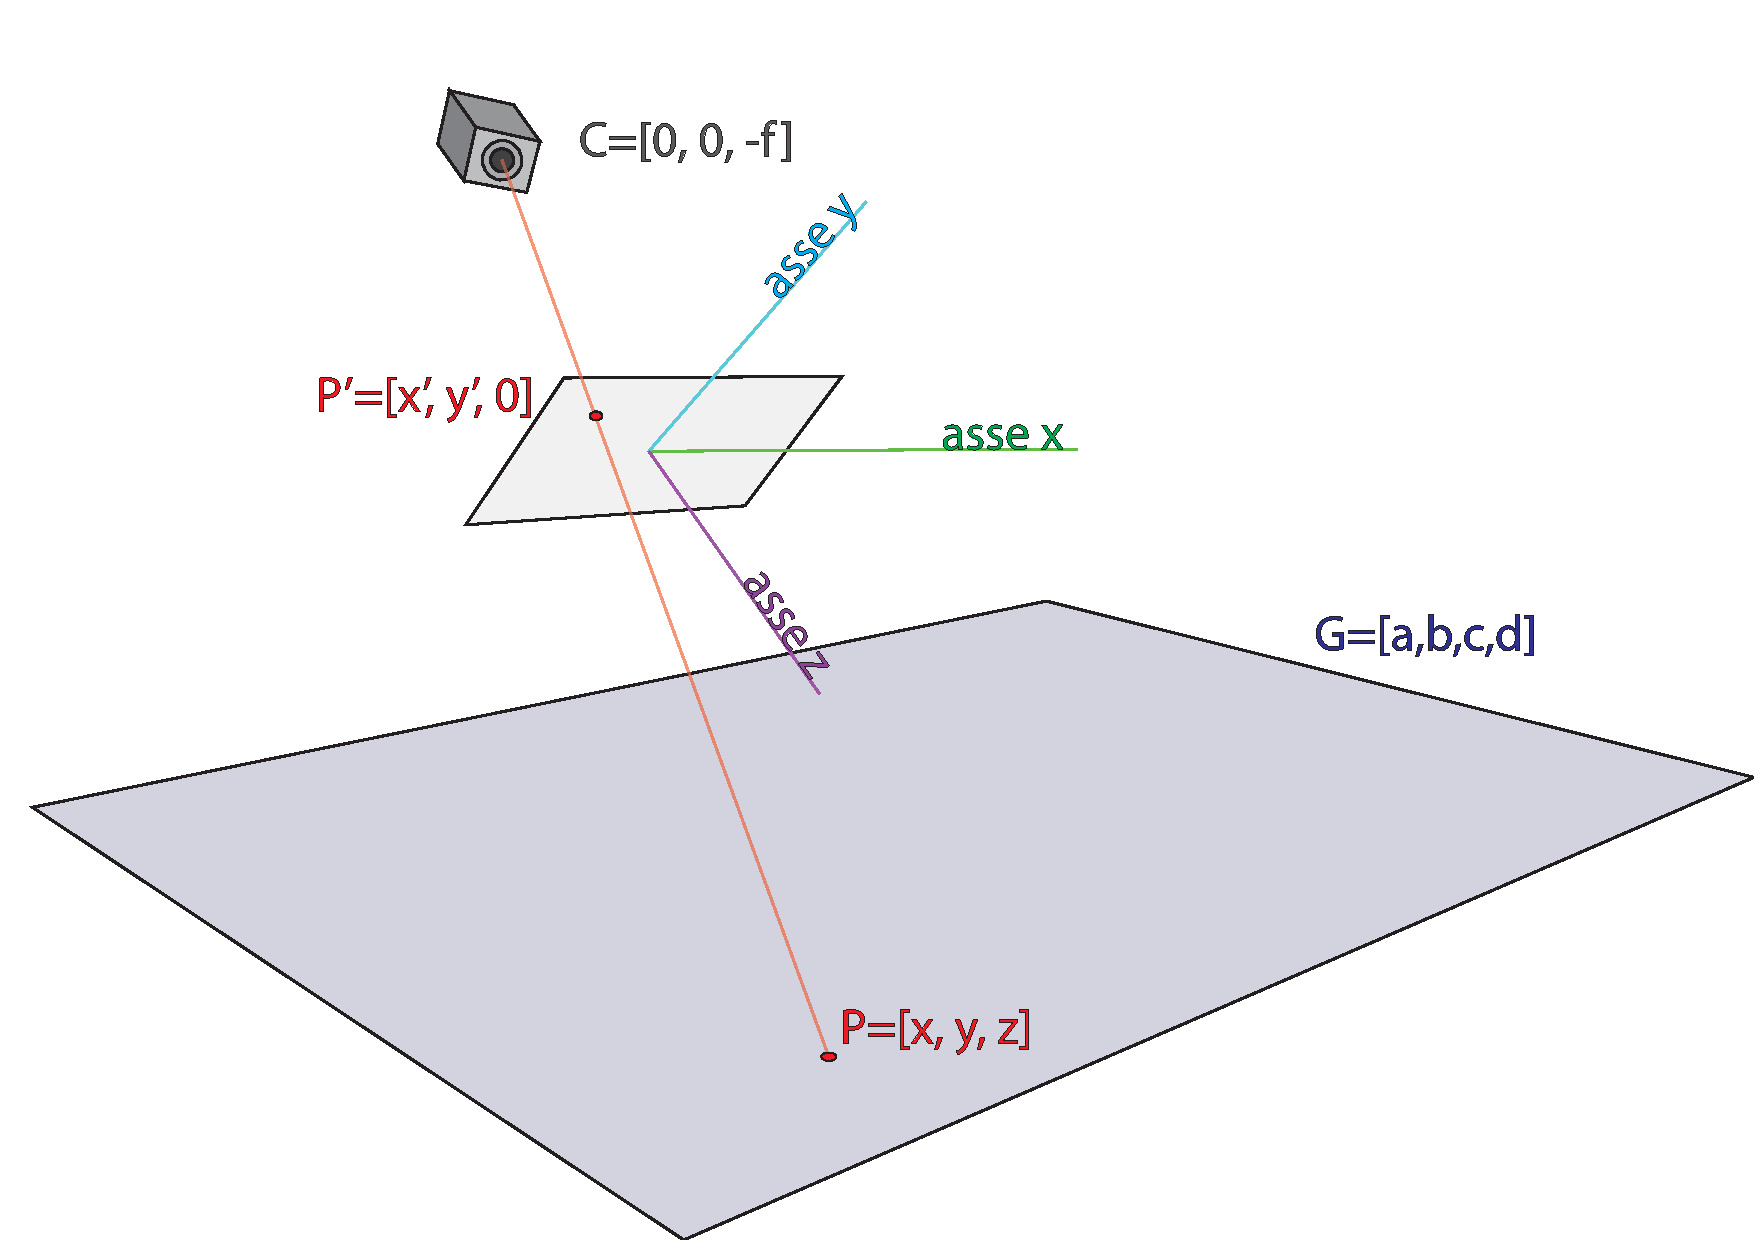
\includegraphics[height=.6\textheight, width=\linewidth, keepaspectratio] 
        { images/camera coords.pdf }

        \vspace{.6em}

        \scalebox{.9} { $
             \begin{bmatrix*}[r]
                cf - d & 0      & 0   \\
                0      & cf - d & 0   \\
                -fa    & -fb    & -fd \\
                a      & b      & cf  \\
            \end{bmatrix*} 
        $ }
    }

    \section{Trasformazione come combinazione}
    \frame{
        \frametitle{\insertsection}

        \parbox[c]{\textwidth}{
        \begin{columns}
            \begin{column}{.33\textwidth}
                \centering
                $P$
                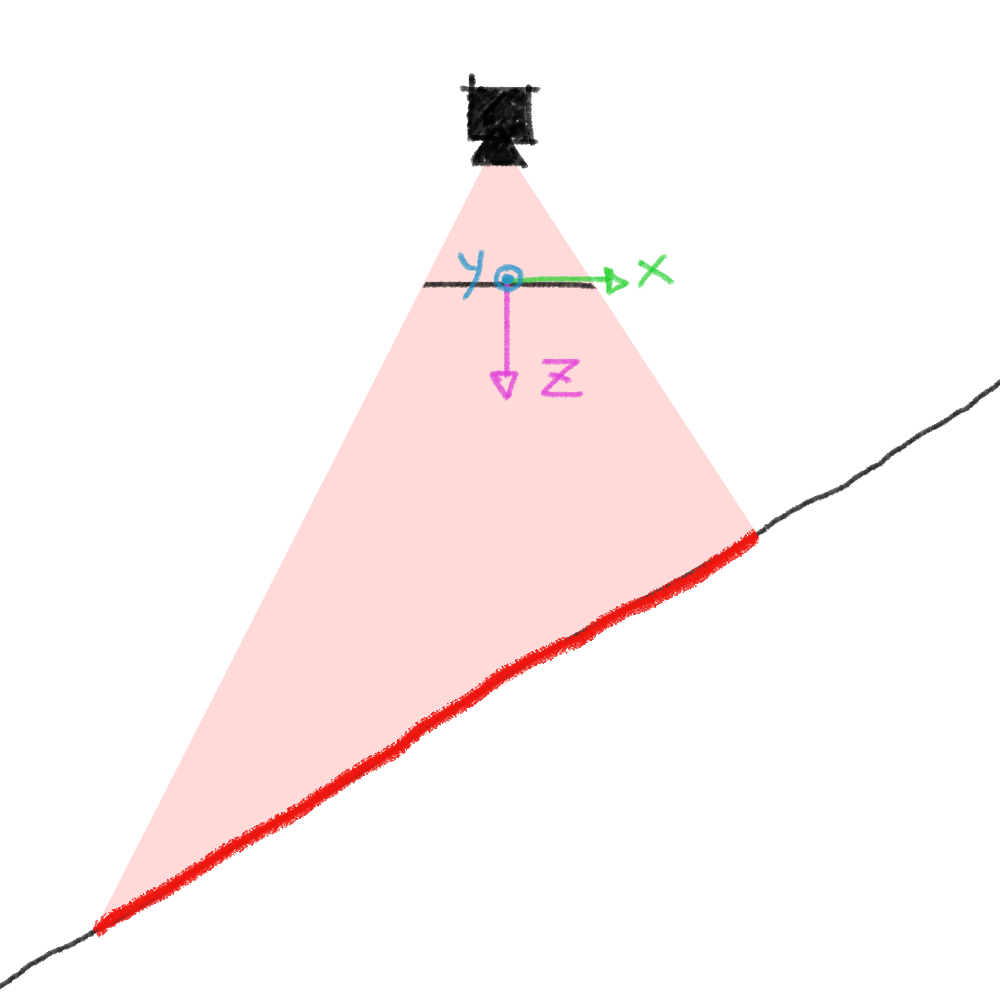
\includegraphics[height=\textheight, width=\textwidth, keepaspectratio]
                { images/P.png } 
            \end{column}
            \begin{column}{.33\textwidth}
                \centering
                $R$
                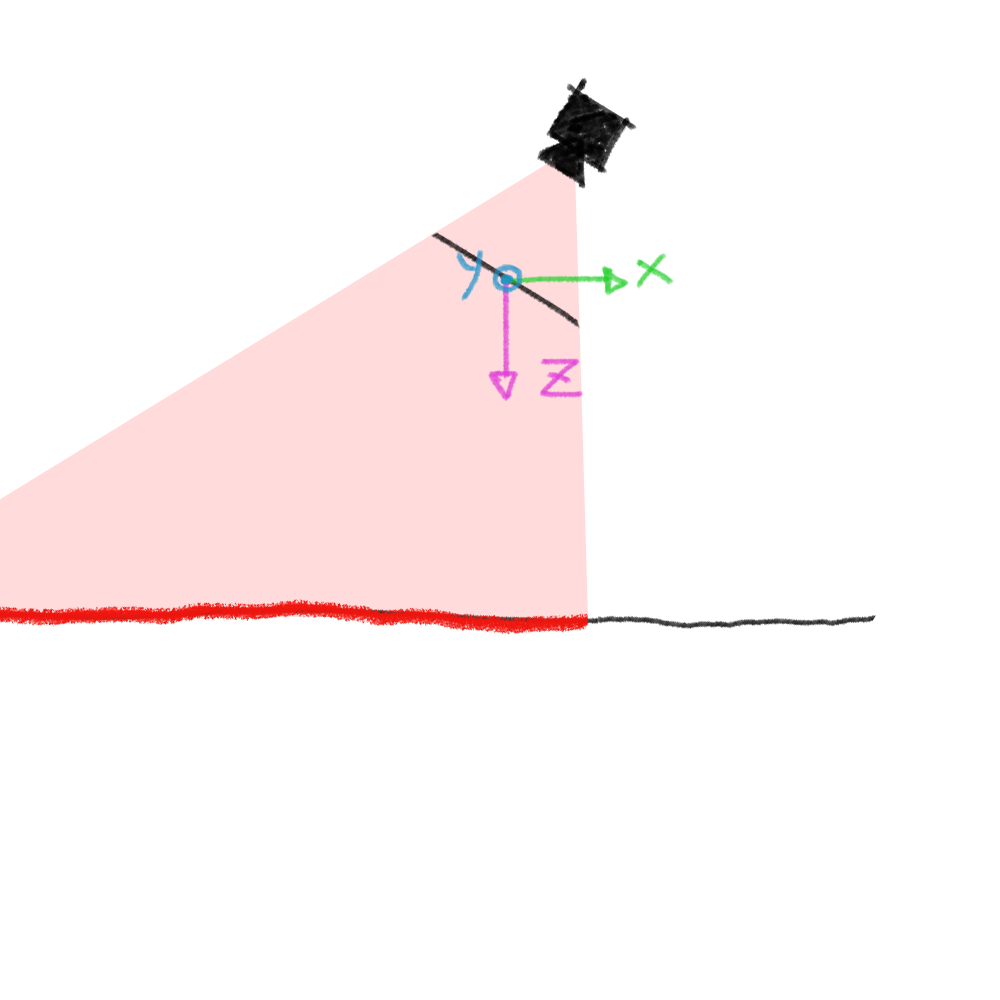
\includegraphics[height=\textheight, width=\textwidth, keepaspectratio]
                { images/R.png } 
            \end{column}
            \begin{column}{.33\textwidth}
                \centering
                $T$ 
                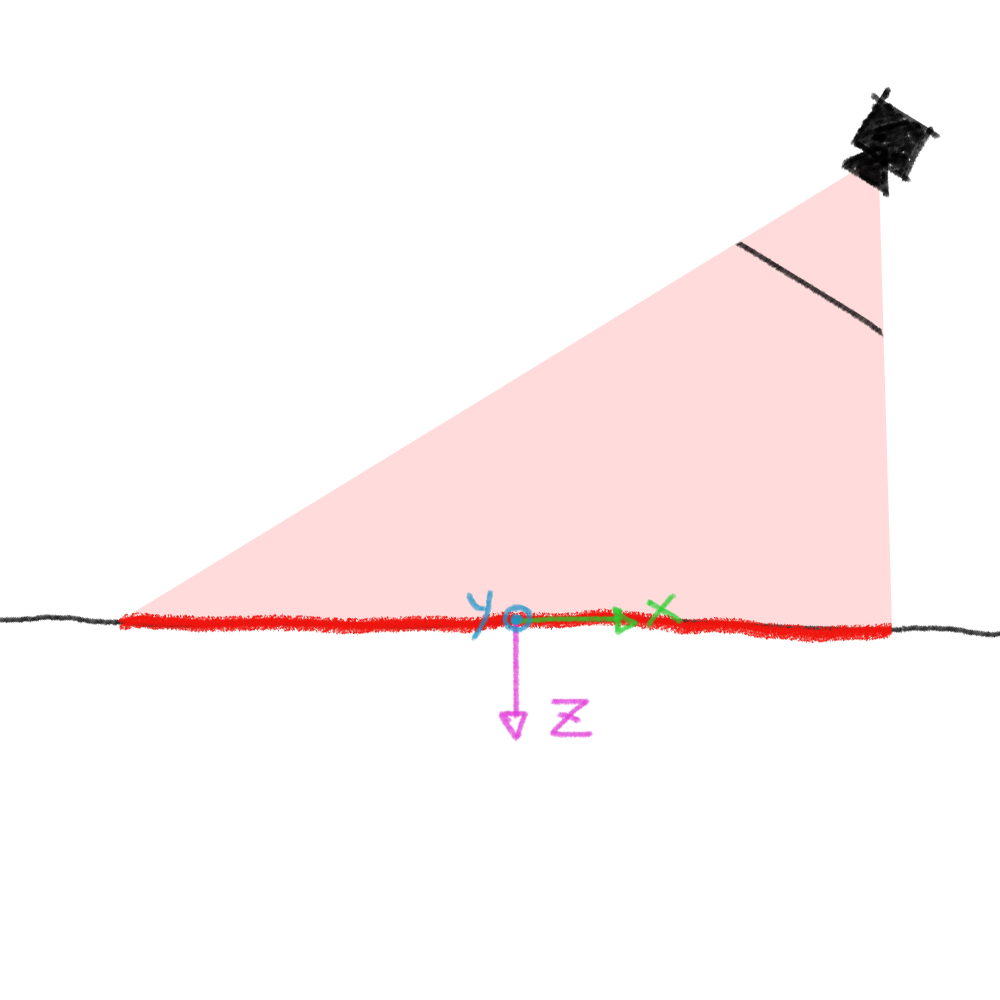
\includegraphics[height=\textheight, width=\textwidth, keepaspectratio]
                { images/T.png } 
            \end{column}
        \end{columns}
        }
        $$
        M = D \cdot T \cdot R \cdot P
        $$
        \begin{center}
            $D = $
            \scalebox{.6}{
                $
                \begin{bmatrix}
                    1 & 0 & 0 & 0 \\
                    0 & 1 & 0 & 0 \\
                    0 & 0 & 0 & 1 \\
                \end{bmatrix}
                $
            }
        \end{center} 
    }

    \section{Da proiezione a posizione}
    \frame{
        \frametitle{\insertsection}
                
        \begin{wrapfigure}[6]{r}{.5\textwidth}
            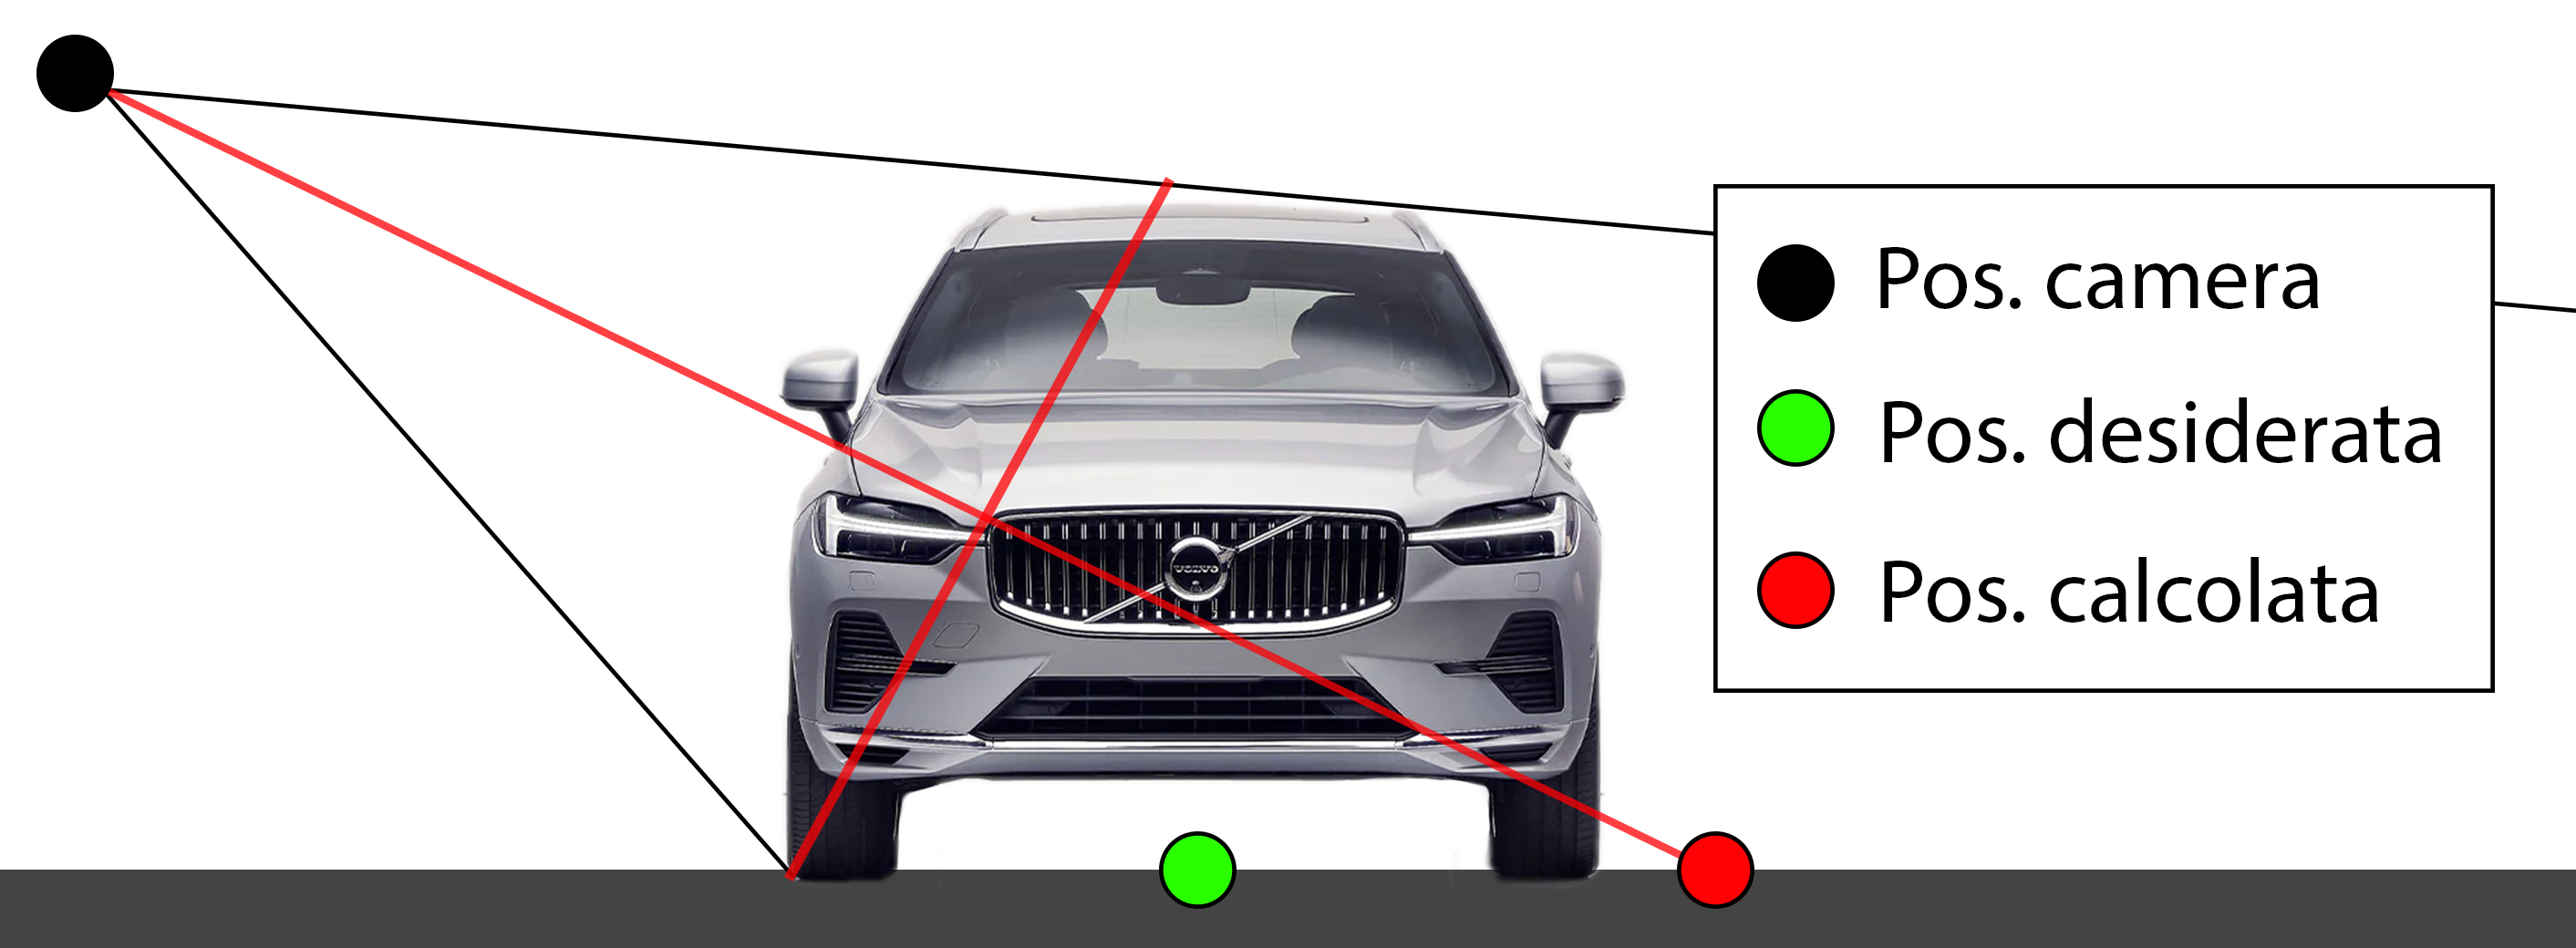
\includegraphics[height=\textheight, width=\linewidth, keepaspectratio]
            { images/proiez_pos.png }
        \end{wrapfigure}

        Proiettare il centro del bounding box non ci da la posizione corretta.
        \vspace{.6em}

        Possiamo proiettare il lato inferiore del bounding box correttamente.
        \vspace{.6em}
        
        Otteniamo una approssimazione migliore utilizzando le dimensioni medie dei veicoli e la loro direzione di movimento.

        \vfill
        \begin{columns}
            \footnotesize
            \itshape
            \begin{column}{.5\textwidth}
                \centering
                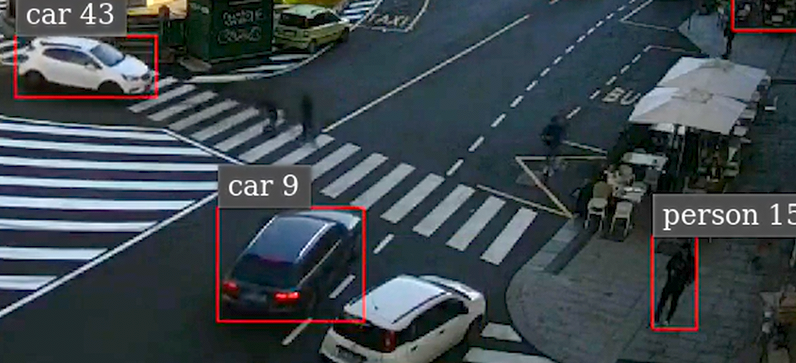
\includegraphics[height=\textheight, width=\textwidth, keepaspectratio]
                { images/yolo.png } \\
                Bounding Boxes
            \end{column}
            \begin{column}{.5\textwidth}
                \centering
                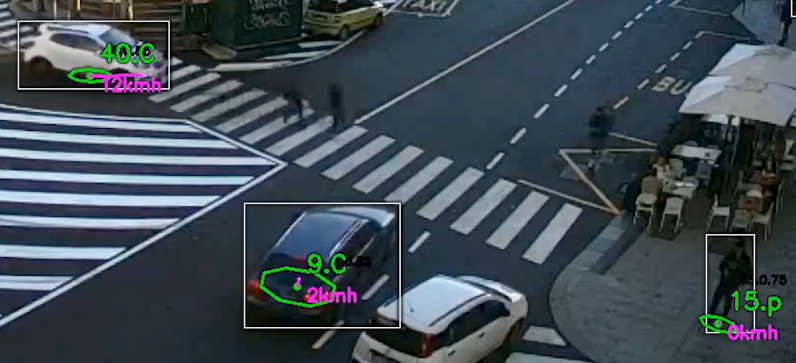
\includegraphics[height=\textheight, width=\textwidth, keepaspectratio]
                { images/corrected.png } \\
                Prospettiva corretta
            \end{column}
        \end{columns}
    }

    \part{Velocità}
    \frame{\partpage}
    \section{Legge del moto e media mobile esponenziale}
    \frame{
        \frametitle{\insertsection}

        Proviamo a calcolare la velocità utilizzando le posizioni trovate e l'equazione:
        $$
        \vec{V}_t = \frac{(\vec{P}_t - \vec{P}_{t-1})}{\Delta}
        $$

        Otteniamo però risultati poco utili, in quanto questa operazione amplifica gli errori presenti nelle misure di posizione.
        \vspace{1.2em}

        Proviamo quindi a correggere questo errore utilizzando una media mobile esponenziale:
        $$
        \vec{V'}_t = k \cdot \vec{V'}_{t-1} + (1-k) \cdot \vec{V}_t
        $$
        Ma anche questo non ci da risultati accettabili.
    }

    \frame{
        \frametitle{\insertsection}
        \centering
        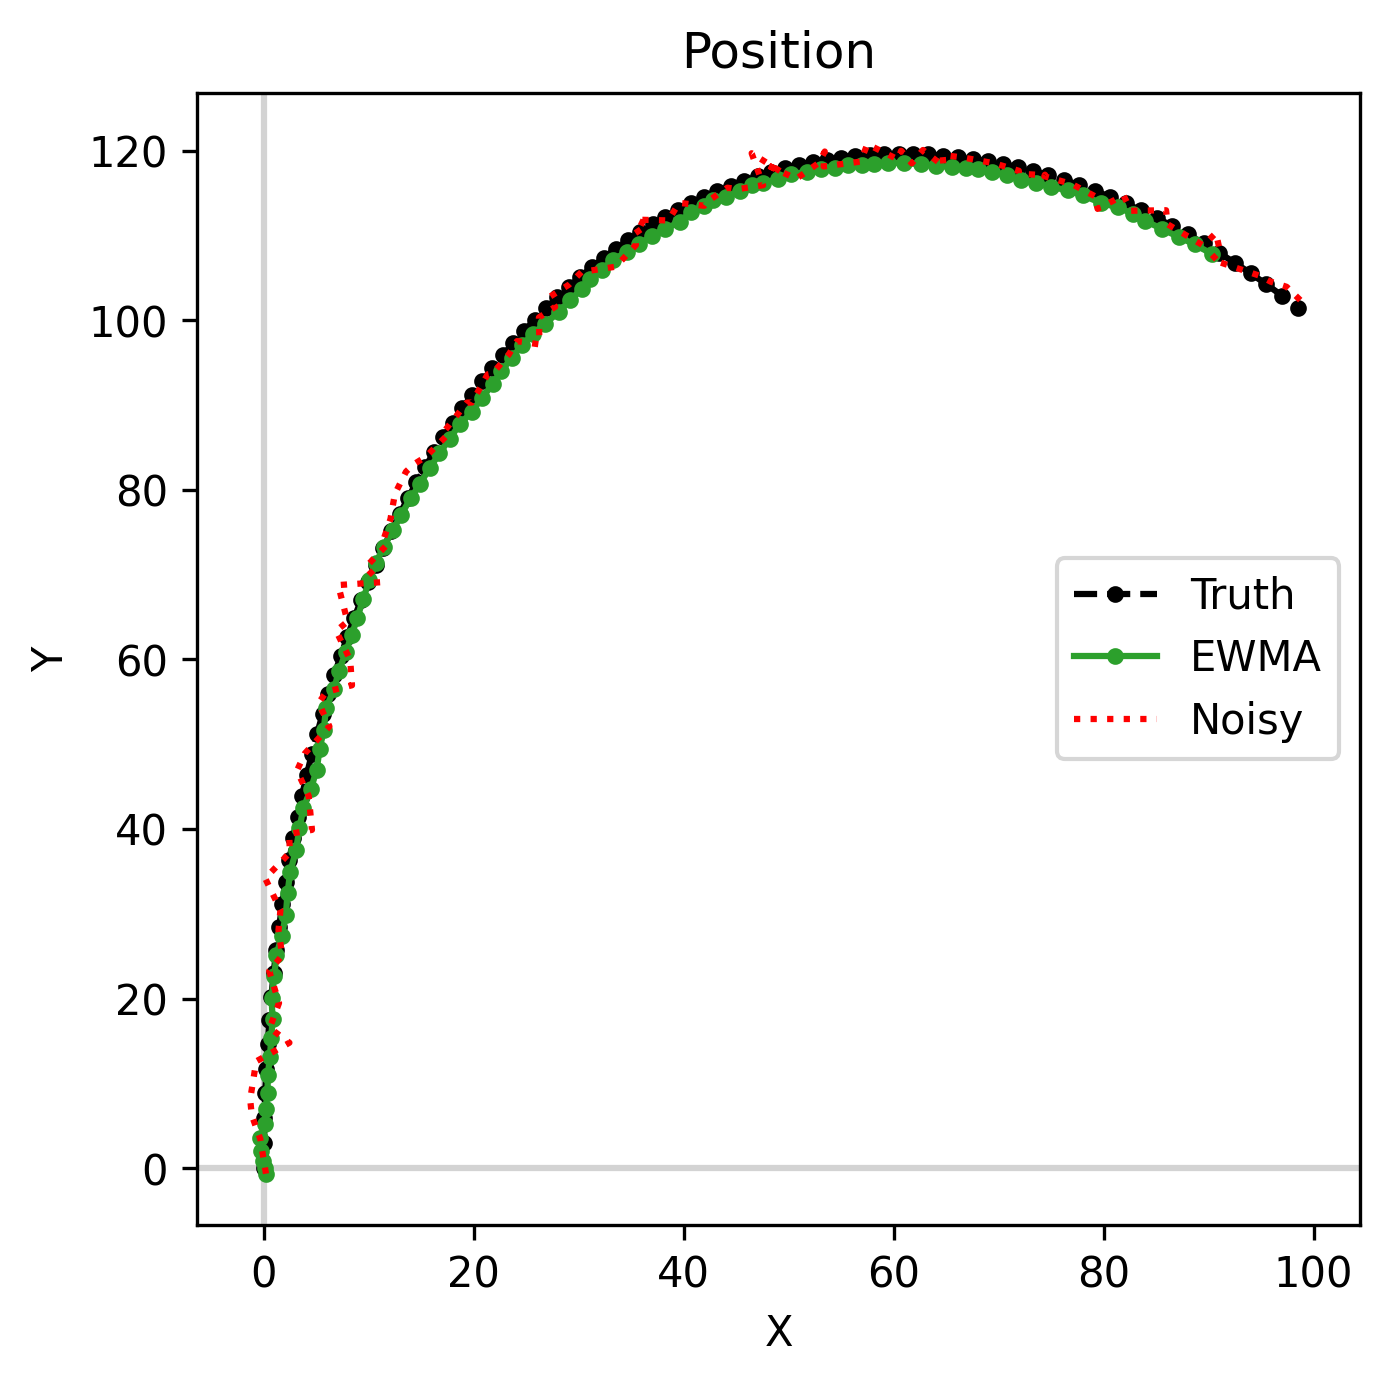
\includegraphics[height=.4\textheight, width=.49\textwidth, keepaspectratio] { images/pos0.png }
        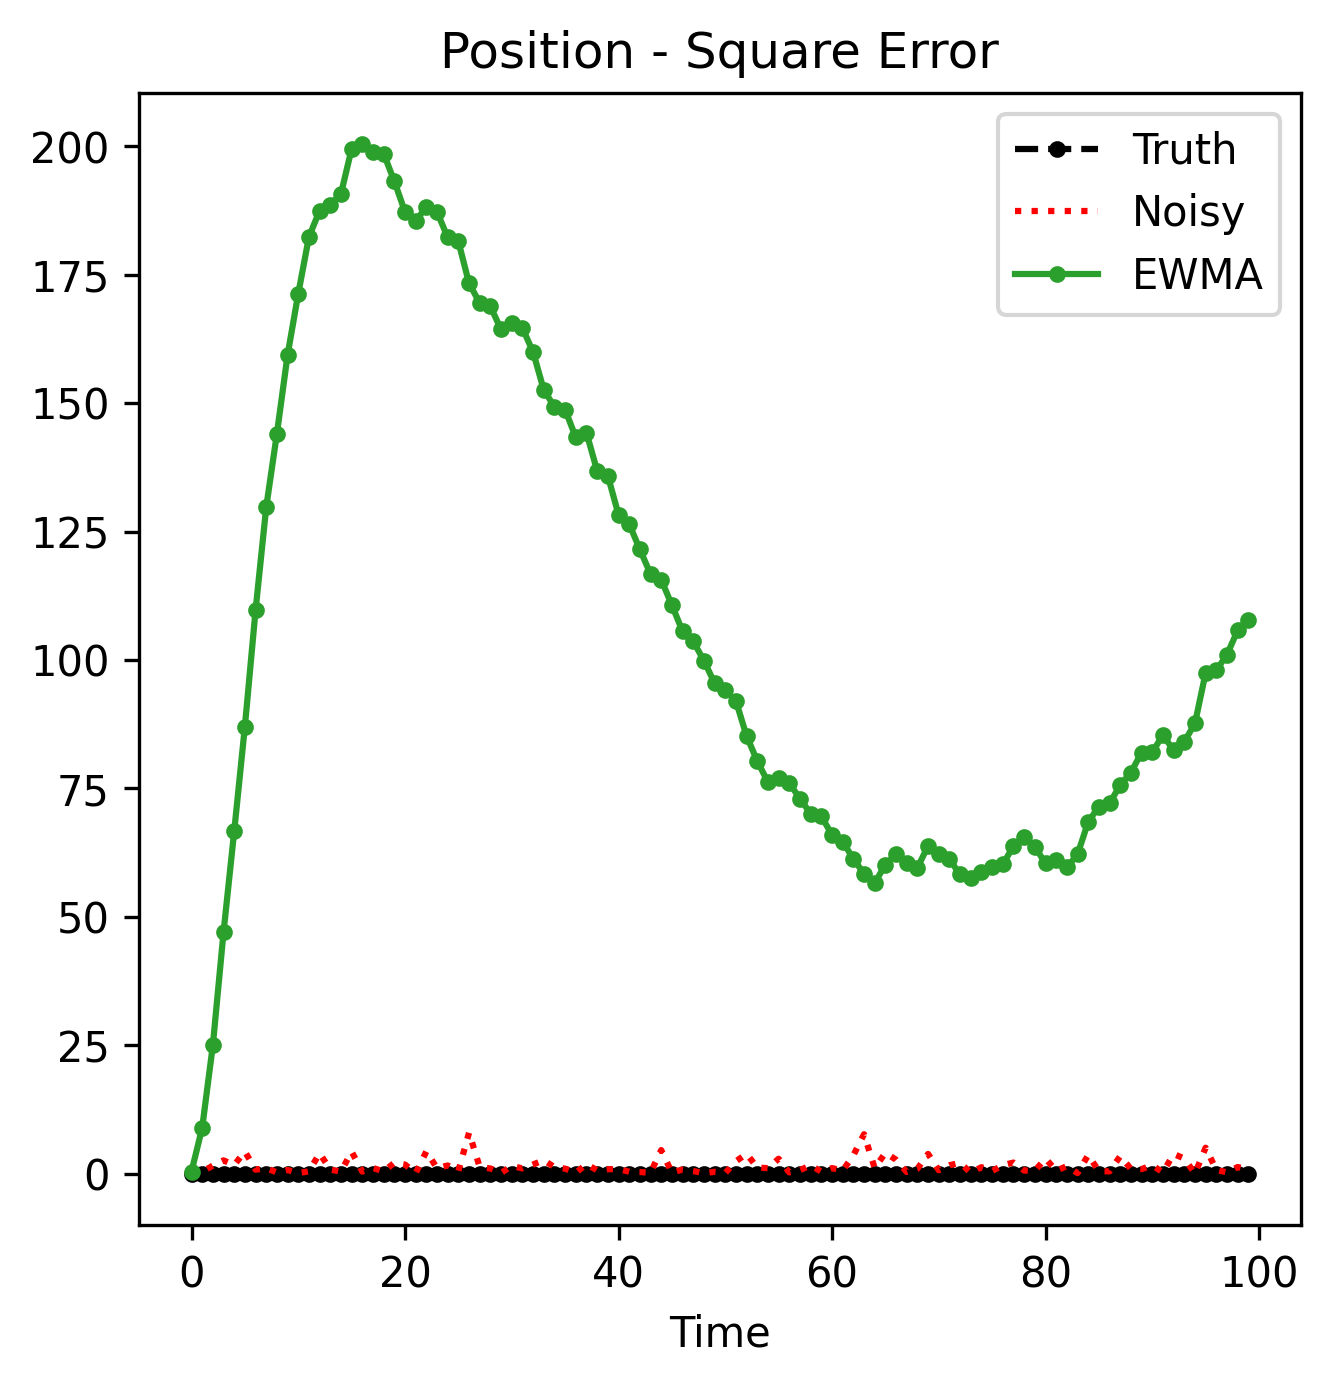
\includegraphics[height=.4\textheight, width=.49\textwidth, keepaspectratio] { images/pos0err.png }
        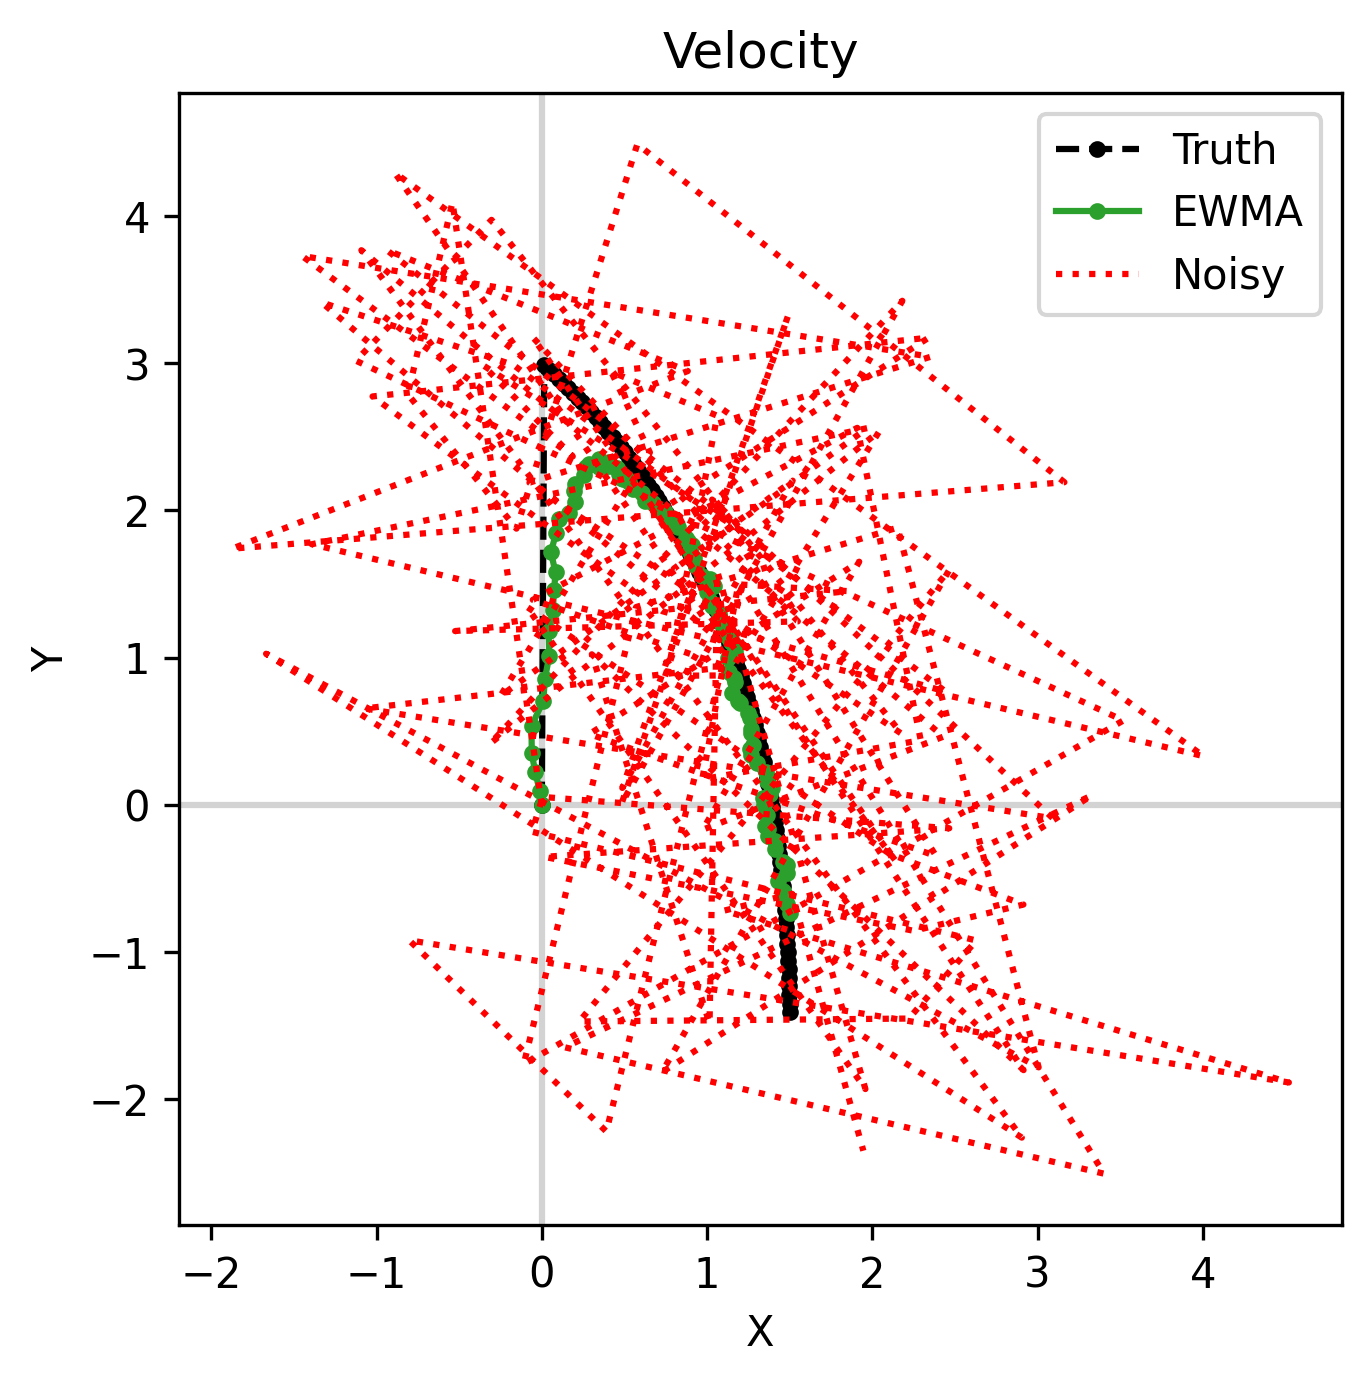
\includegraphics[height=.4\textheight, width=.49\textwidth, keepaspectratio] { images/vel0.png }
        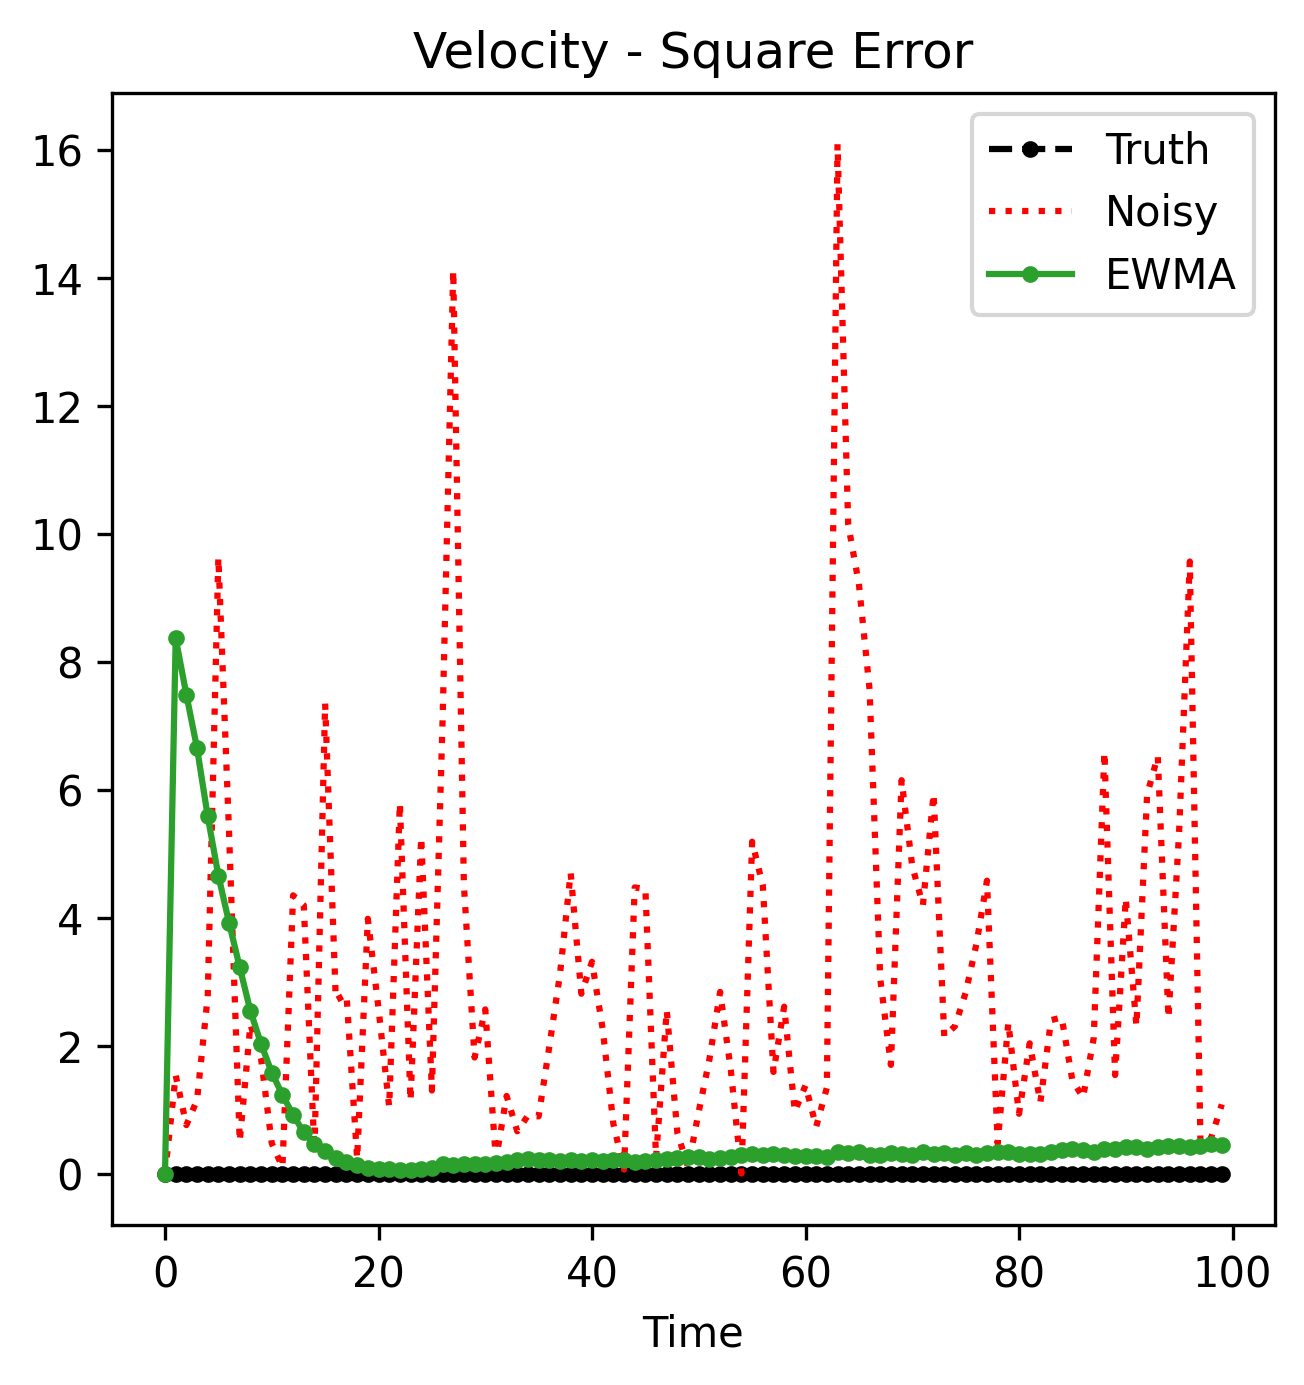
\includegraphics[height=.4\textheight, width=.49\textwidth, keepaspectratio] { images/vel0err.png }
    }

    \section{Il nostro algoritmo}
    \frame{
        \frametitle{\insertsection}
        Abbiamo quindi bisogno di un algoritmo che ci permetta di calcolare la velocità correggendo l'errore.
        \vspace{1.2em}

        Gli algoritmi più utilizzati sono il Kalman Filter e le sue estensioni, ma questi sono difficili da comprendere e implementare correttamente.
        \vspace{1.2em}

        Proponiamo quindi un nuovo algoritmo e lo confrontiamo con un algoritmo proposto in letteratura come alternativa al Kalman Filter.
    }
    \frame{
        \frametitle{\insertsection}
        \begin{equation*}
        \begin{split}
            & p'_t = p_{t-1} + v_{t-1} + \frac{1}{2} \cdot a_{t-1} \\
            & v'_t = v_{t-1} + a_{t-1} \\
            & \\
            & p_t = k \cdot p'_t + (1-k) \cdot P_t \\
            & v_t = k \cdot v'_t + (1-k) \cdot (p_t - p'_t) \\
            & a_t = k \cdot a_{t-1} + (1-k) \cdot (v_t - v'_t) \\
            & \\
            & P'_t = p_t + v_t \cdot \left(\frac{k}{1-k}\right) + \frac{1}{2} \cdot a_t \cdot \left(\frac{k}{1-k}\right)^2 \\
            & V'_t = 2 \cdot \left(v_t + a_t \cdot \left(\frac{k}{1-k}\right)\right)
        \end{split}
        \end{equation*}
    }

    \section{L'algoritmo di confronto}
    \frame{
        \frametitle{\insertsection}

        \textbf{\emph{Double Exponential Smoothing: An Alternative to Kalman Filter-Based Predictive Tracking - J. LaViola Jr. 2003}}

        \begin{equation*}
            \begin{split}
                & Sp_t = \alpha \cdot P_t + (1-\alpha) \cdot Sp_{t-1} \\
                & Sp^{[2]}_t = \alpha \cdot Sp_{t} + (1-\alpha) \cdot Sp^{[2]}_{t-1} \\
                & \\
                & P'_T = \left(2 + \frac{\alpha \cdot \tau}{1 - \alpha}\right) \cdot Sp_t - \left(1 + \frac{\alpha \cdot \tau}{1 - \alpha}\right) \cdot Sp^{[2]}_t \\
            \end{split}
        \end{equation*}
        \vspace{.6em}

        Per confrontarlo con il nostro algoritmo:
        \begin{itemize}
            \item $\alpha = 1 - k$
            \item $T = t + \tau$ e quindi $\tau = 0 \rightarrow  T = t$
        \end{itemize}
    }

    \section{Risultati}
    \frame{
        \frametitle{\insertsection}
        \centering
        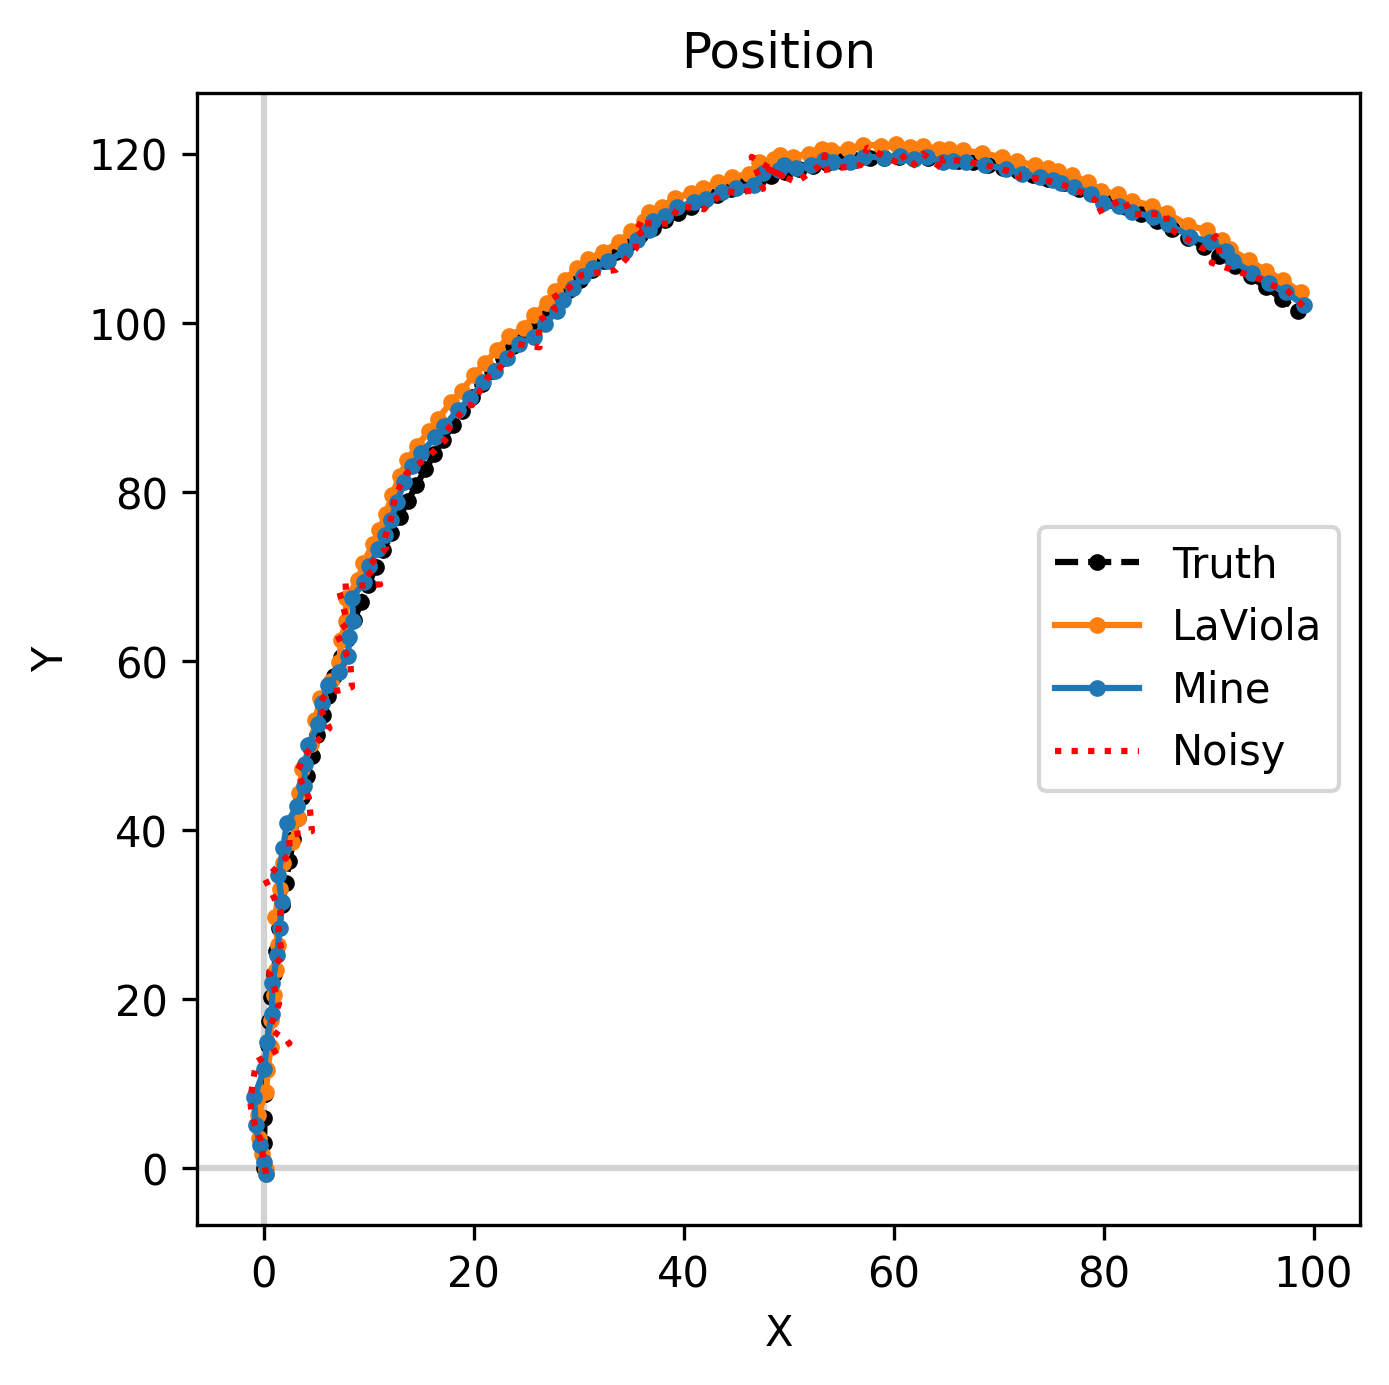
\includegraphics[height=.4\textheight, width=.49\textwidth, keepaspectratio] { images/pos1.png }
        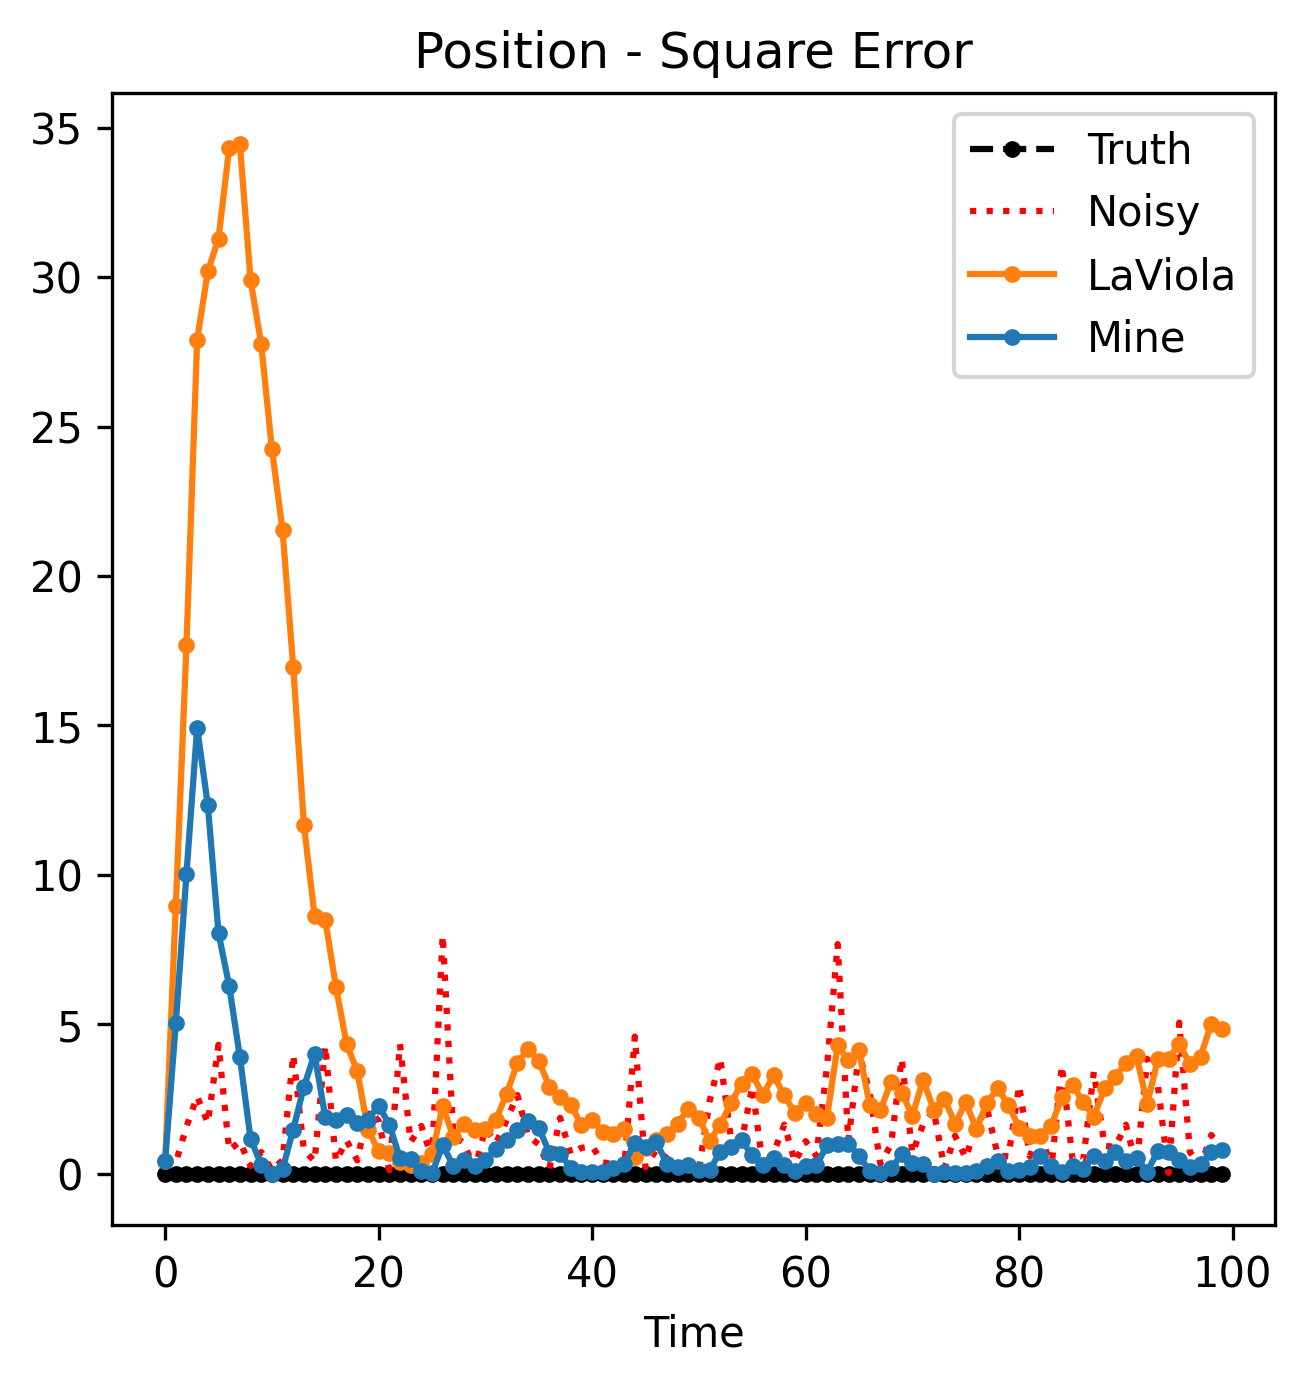
\includegraphics[height=.4\textheight, width=.49\textwidth, keepaspectratio] { images/pos1err.png }
        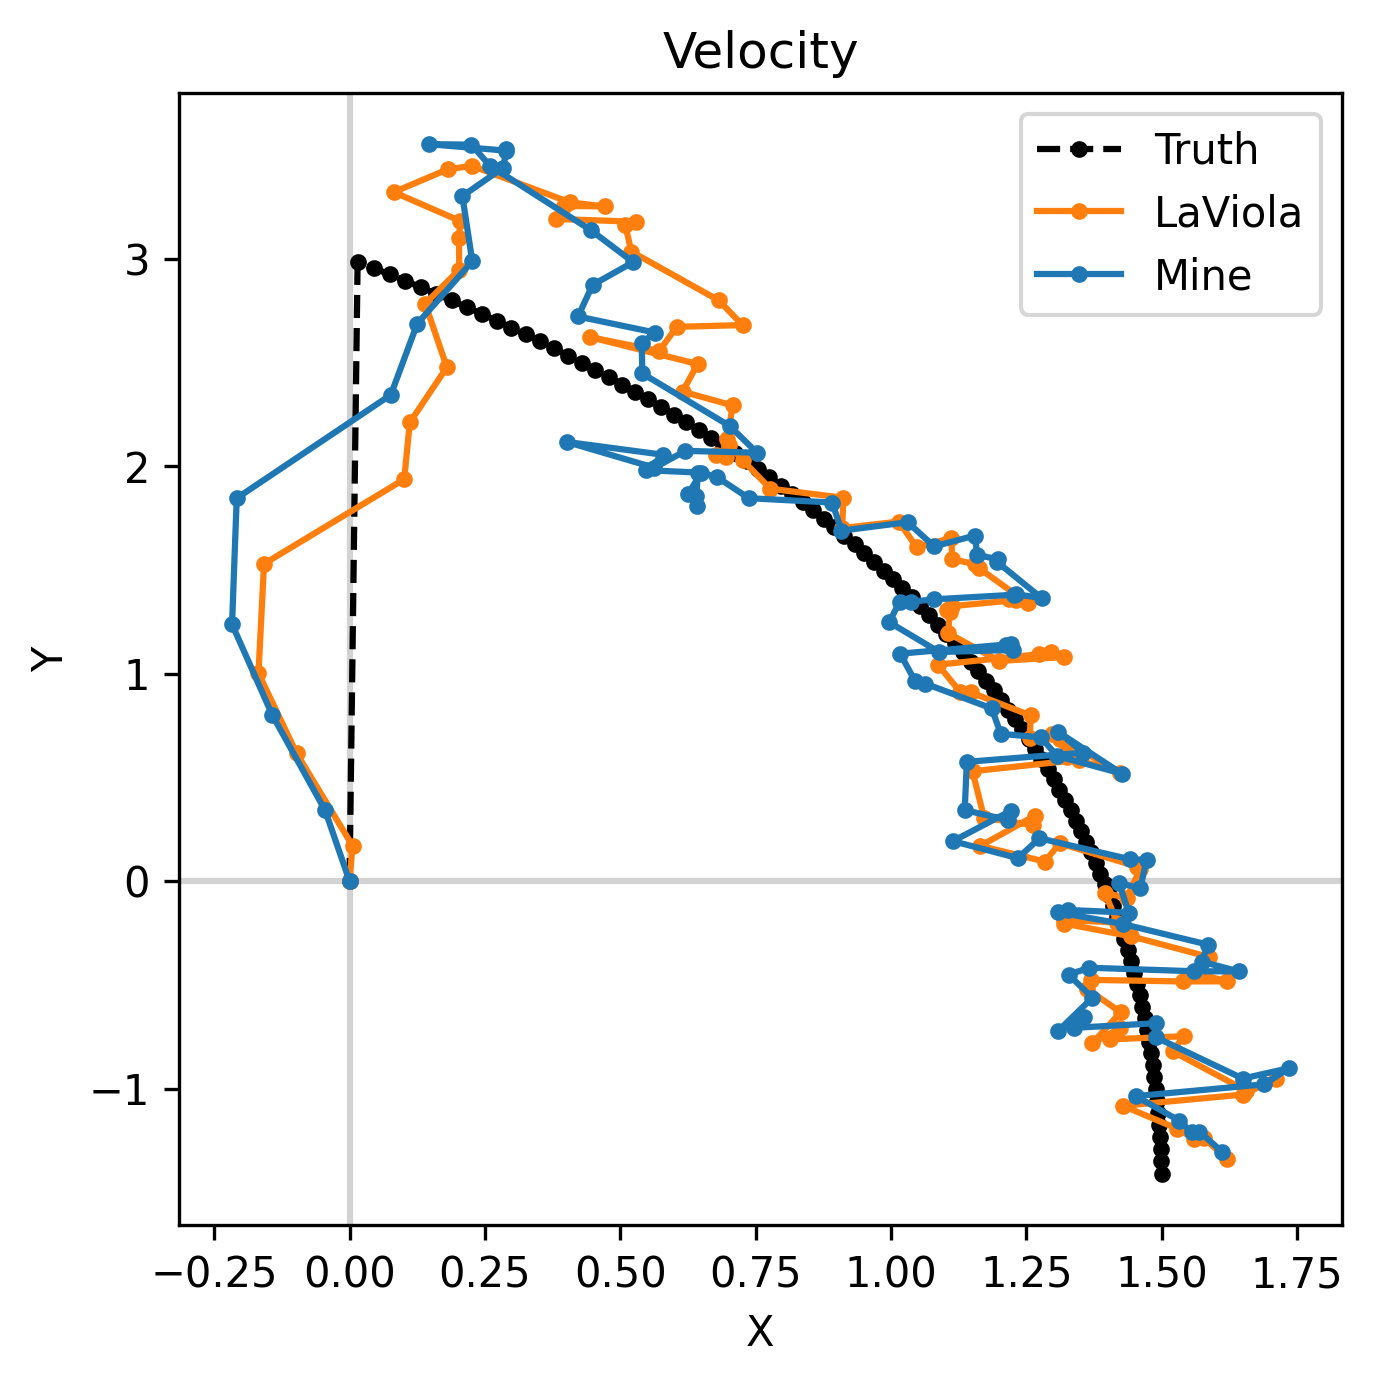
\includegraphics[height=.4\textheight, width=.49\textwidth, keepaspectratio] { images/vel1.png }
        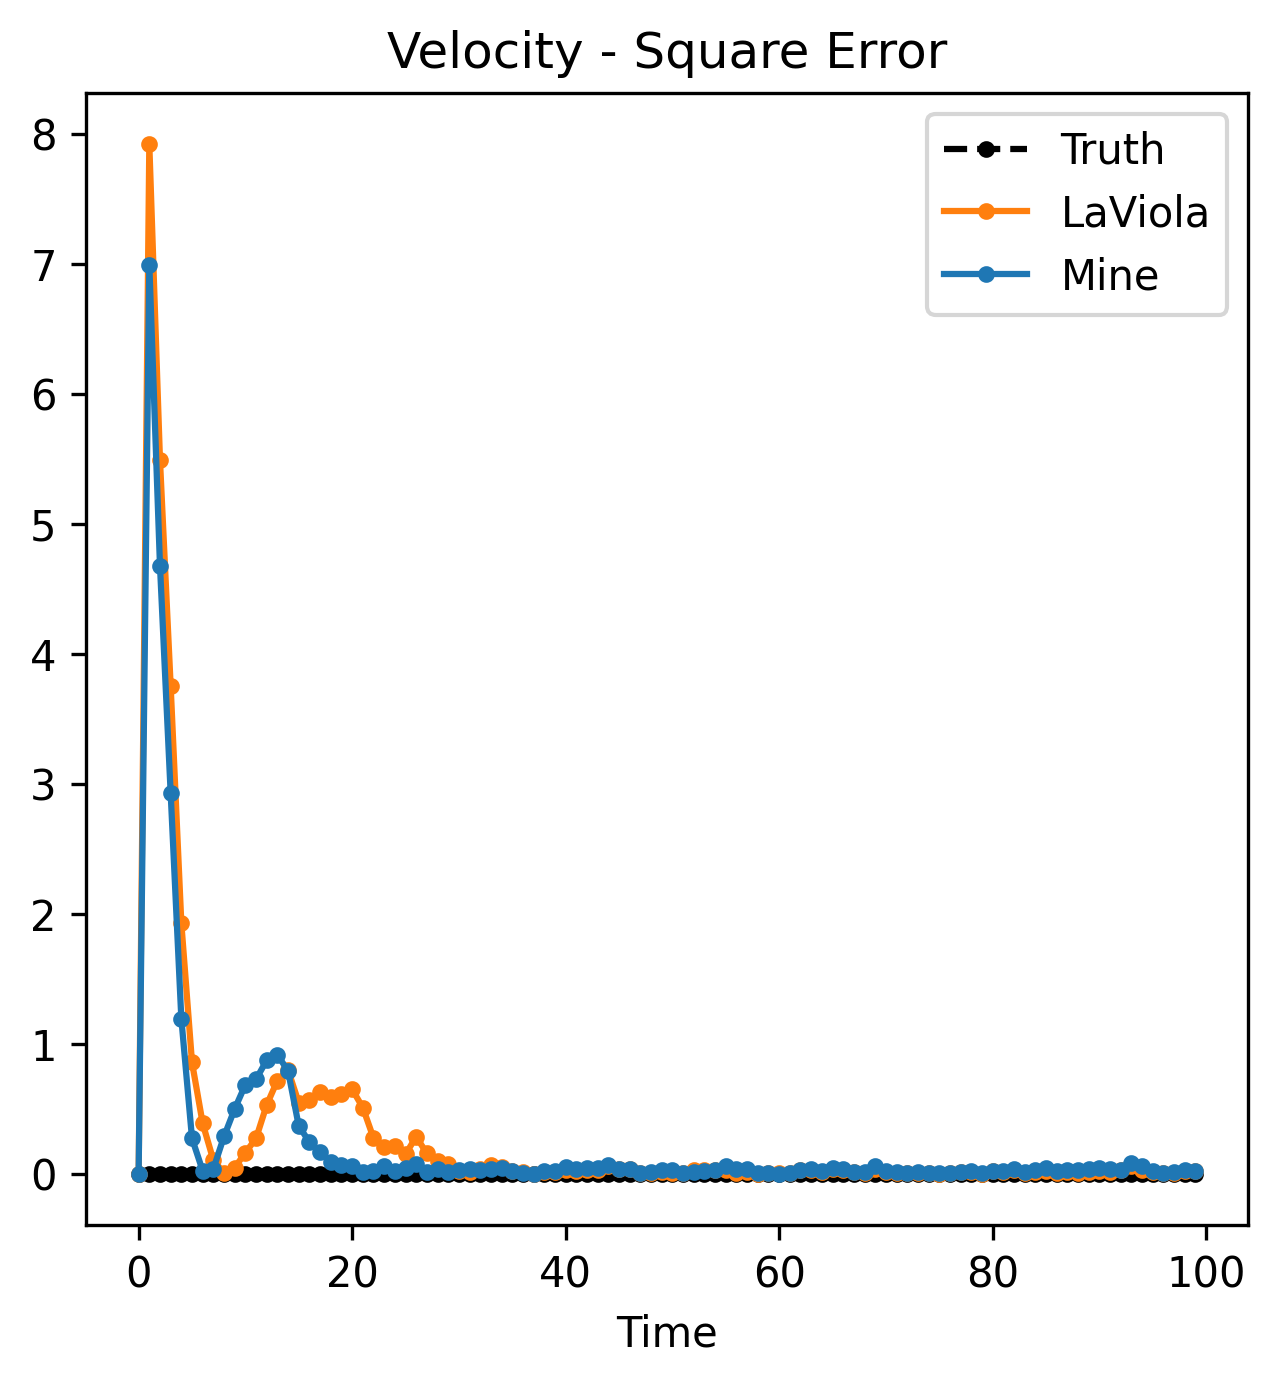
\includegraphics[height=.4\textheight, width=.49\textwidth, keepaspectratio] { images/vel1err.png }
    }

    \frame{
        \frametitle{\insertsection}
        \begin{table}
            \caption{Posizione: Errore quadrato medio}
            \centering
            \begin{subtable}{.49\textwidth}
                \caption{da $t=0$}
                \centering
                \begin{tabular}{l r}
                    Rumore &    1.5255 \\
                    EWMA &    107.4193 \\
                    LaViola &   5.3685 \\
                    Nostro &    1.2012 \\
                \end{tabular}
            \end{subtable}
            \hfill
            \begin{subtable}{.49\textwidth}
                \caption{ da $t=20$ }
                \centering
                \begin{tabular}{l r}
                    Rumore &   1.5578 \\
                    EWMA &   100.6619 \\
                    LaViola &  2.3364 \\
                    Nostro &   0.5000 \\
                \end{tabular}
            \end{subtable}
        \end{table}
        \begin{table}
            \caption{Velocità: Errore quadrato medio}
            \centering
            \begin{subtable}{.49\textwidth}
                \caption{da $t=0$}
                \centering
                \begin{tabular}{l r}
                    Rumore  & 3.0807 \\
                    EWMA    & 0.7228 \\
                    LaViola & 0.2980 \\
                    Nostro  & 0.2397 \\
                \end{tabular}
            \end{subtable}
            \hfill
            \begin{subtable}{.49\textwidth}
                \caption{ da $t=20$ }
                \centering
                \begin{tabular}{l r}
                    Rumore  & 3.1961 \\
                    EWMA    & 0.2744 \\
                    LaViola & 0.0484 \\
                    Nostro  & 0.0267 \\
                \end{tabular}
            \end{subtable}
        \end{table}
    }
    
    \part{Sistema e conclusioni}
    \frame{\partpage}
    \section{Sistema}
    \frame{
        \frametitle{\insertsection}
        \centering
        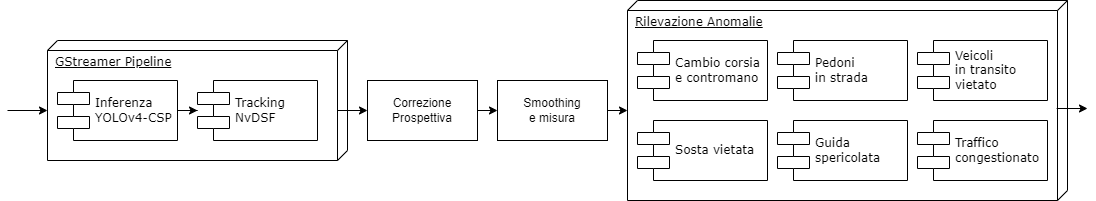
\includegraphics[height=\textheight, width=\textwidth, keepaspectratio]
        { images/arch.png }
    }
    \section{Conclusioni}
    \frame{
        \frametitle{\insertsection}
    }
\end{document}
